% ------------------------------------------------------------------------------
% TYPO3 Version 9.1 - What's New - Chapter "Backend User Interface" (English Version)
%
% @author	Michael Schams <schams.net>
% @license	Creative Commons BY-NC-SA 3.0
% @link		http://typo3.org/download/release-notes/whats-new/
% @language	English
% ------------------------------------------------------------------------------
% LTXE-CHAPTER-UID:		07b25346-95b1df21-a6ebe09a-49f53f41
% LTXE-CHAPTER-NAME:	Backend User Interface
% ------------------------------------------------------------------------------

\section{Backend User Interface}
\begin{frame}[fragile]
	\frametitle{Backend User Interface}

	\begin{center}\huge{Kapitel 1:}\end{center}
	\begin{center}\huge{\color{typo3darkgrey}\textbf{Backend User Interface}}\end{center}

\end{frame}

% ------------------------------------------------------------------------------
% LTXE-SLIDE-START
% LTXE-SLIDE-UID:		96e449d4-a887ec58-fe155dde-007dbcb7
% LTXE-SLIDE-TITLE:		Duplicate Content Element
% LTXE-SLIDE-REFERENCE:	Feature-77685-CreateASaveAndOpenCopyButtonWhenSavingAContentElement
% ------------------------------------------------------------------------------

\begin{frame}[fragile]
	\frametitle{Backend User Interface}
	\framesubtitle{Duplicate Content Element}

	Backend Benutzer (z.B. Redakteure) können ein Inhaltselement ganz einfach mit einem Klick auf "duplicate" klonen.

	\begin{figure}
		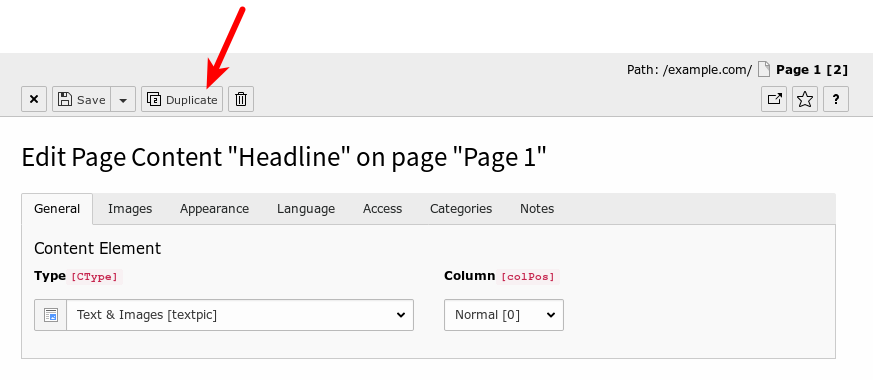
\includegraphics[width=0.9\linewidth]{BackendUserInterface/DuplicateContentElementButton.png}
	\end{figure}

\end{frame}

% ------------------------------------------------------------------------------
% LTXE-SLIDE-START
% LTXE-SLIDE-UID:		d2c39382-667704b2-fb81bb2e-4d59183e
% LTXE-SLIDE-TITLE:		Show Value of Fields
% LTXE-SLIDE-REFERENCE:	Feature-83748-ShowValueOfFieldsInDebugMode
% ------------------------------------------------------------------------------

\begin{frame}[fragile]
	\frametitle{Backend User Interface}
	\framesubtitle{Wert der Felder anzeigen}

	Im Debug-Modus (\texttt{\$GLOBALS['TYPO3\_CONF\_VARS']['BE']['debug']}),
	werden die Werte der Felder in eckigen Klammern angezeigt. Dies sind die
	\textit{reale} Werte die in der Datenbank eingetragen sind (nur für BE administrator
	Benutzer).

	\begin{figure}
		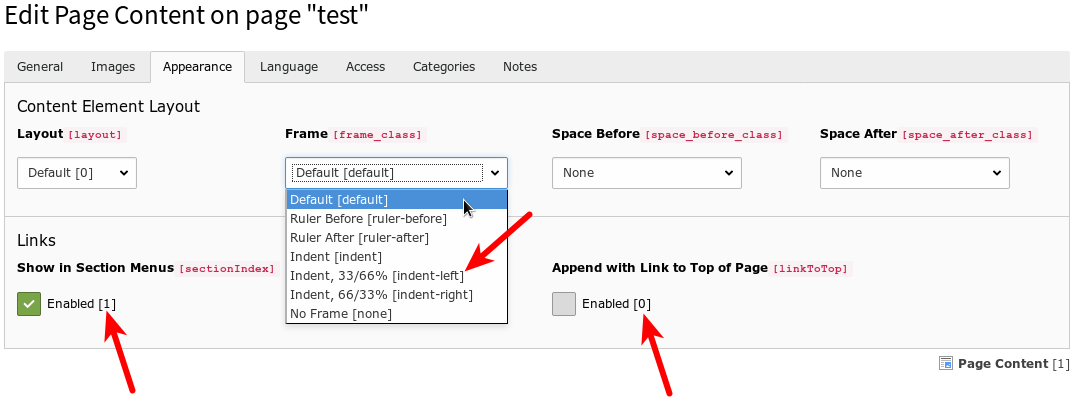
\includegraphics[width=0.9\linewidth]{BackendUserInterface/ShowValueOfFieldsInDebugMode.png}
	\end{figure}

\end{frame}

% ------------------------------------------------------------------------------
% LTXE-SLIDE-START
% LTXE-SLIDE-UID:		7922e712-da1f1937-50e83e2d-0395df58
% LTXE-SLIDE-TITLE:		Create task group from add/edit task form
% LTXE-SLIDE-REFERENCE:	Feature-69187-EXTSchedulerCreateTaskGroupFromAddeditTaskForm
% ------------------------------------------------------------------------------

\begin{frame}[fragile]
	\frametitle{Backend User Interface}
	\framesubtitle{Scheduler Task Group}

	Eine neue Schedular Task Gruppe kann beim Bearbeiten oder Erstellen einer Aufgabe erstellt werden.
	Es ist nicht mehr notwendig zum Listenmodul zu wechseln.

	\begin{figure}
		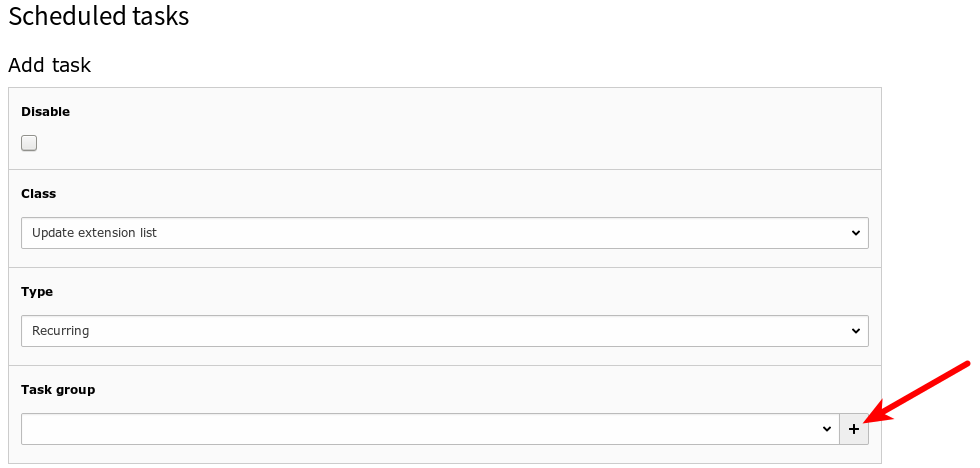
\includegraphics[width=0.8\linewidth]{BackendUserInterface/SchedulerCreateTaskGroupFromAddeditTaskForm.png}
	\end{figure}

\end{frame}

% ------------------------------------------------------------------------------
% LTXE-SLIDE-START
% LTXE-SLIDE-UID:		7922e712-da1f1937-50e83e2d-0395df58
% LTXE-SLIDE-TITLE:		FormEngine: Checkbox Toggle Switches
% LTXE-SLIDE-REFERENCE:	Feature-83556-AddToggleSwitchesToFormEngine
% ------------------------------------------------------------------------------

\begin{frame}[fragile]
	\frametitle{Backend User Interface}
	\framesubtitle{Checkbox-Klippschalter}

	Checkbox-Klippschalter ermöglichen BE-Benutzer den einfachen Wechsel zwischen Zuständen.

	\begin{figure}
		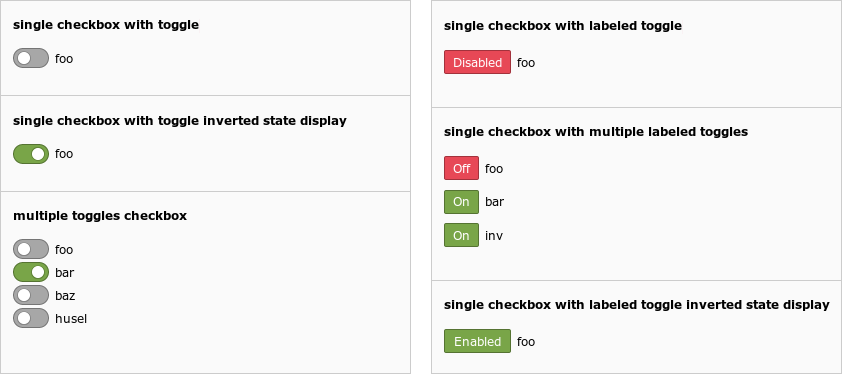
\includegraphics[width=0.9\linewidth]{BackendUserInterface/AddToggleSwitchesToFormEngine.png}
	\end{figure}

\end{frame}

% ------------------------------------------------------------------------------
